\documentclass[a4paper,leqno]{article}

\usepackage[T1]{fontenc}
\usepackage[utf8]{inputenc}
\usepackage[english]{babel}
\usepackage{amsmath}
\usepackage{longtable} 
\usepackage{multirow} 
\usepackage{graphicx}
\usepackage{algorithm2e}
\usepackage{listings}

\begin{document}
	
	
\date{2017/11/26}
\author{Bolshakova Liubov\\ Campagnoli Chiara\\ Lagni Luca}
\title{\textbf{\huge Travlendar+}\\ Design Document}
\begin{minipage}[!t]{\linewidth}
	\centering
	
\includegraphics[scale=0.8]{logo2}
\end{minipage}
\begin{minipage}[!h]{\linewidth}
	\maketitle 
\end{minipage}

\newpage
\tableofcontents                  
  
\newpage	
\section{Introduction}
\subsection{Purpose}
\subsection{Scope}

\subsection{Definitions, Acronyms, Abbreviations}
\begin{itemize}
	\item API: Application Programming Interface.
	\item DD: Design Document
	\item GPS: Global Positioning System.
	\item GSM: Global System for Mobile Communications.
	\item GUI: Graphical User Interface.
	\item OAMOT: Other Autonomous Means of Transport
	\item ONAMOT: Other Non-Autonomous Means of Transport
	\item OS: Operating System.
	\item RAM: Random-access memory.
	\item RASD: Requirement analysis and Specification Document.
	\item SMS: Short Message Service.
\end{itemize}

\subsection{Revision history}
\begin{itemize}
	\item Mandatory Project Assignments.pdf
	\item Requirements Analysis and Specification Document
	\item Design Deliverable Sample from A.Y. 2015-2016.pdf
	\item DD From the car sharing project.pdf
	\item Integration and test plan from the car sharing project.pdf
\end{itemize}

\subsection{Reference Documents}
\subsection{Document Structure}

\newpage
\section{Architectural design}

\subsection{Overview}
Travlendar+ is based on a three-tier architecture. A diagram of the proposed system was already present in section 2.4.3 of the RASD; here we provide on the same diagram a division between the different tiers and a more detailed description of each one of these.

\begin{figure}[!h]
	\begin{centering}
		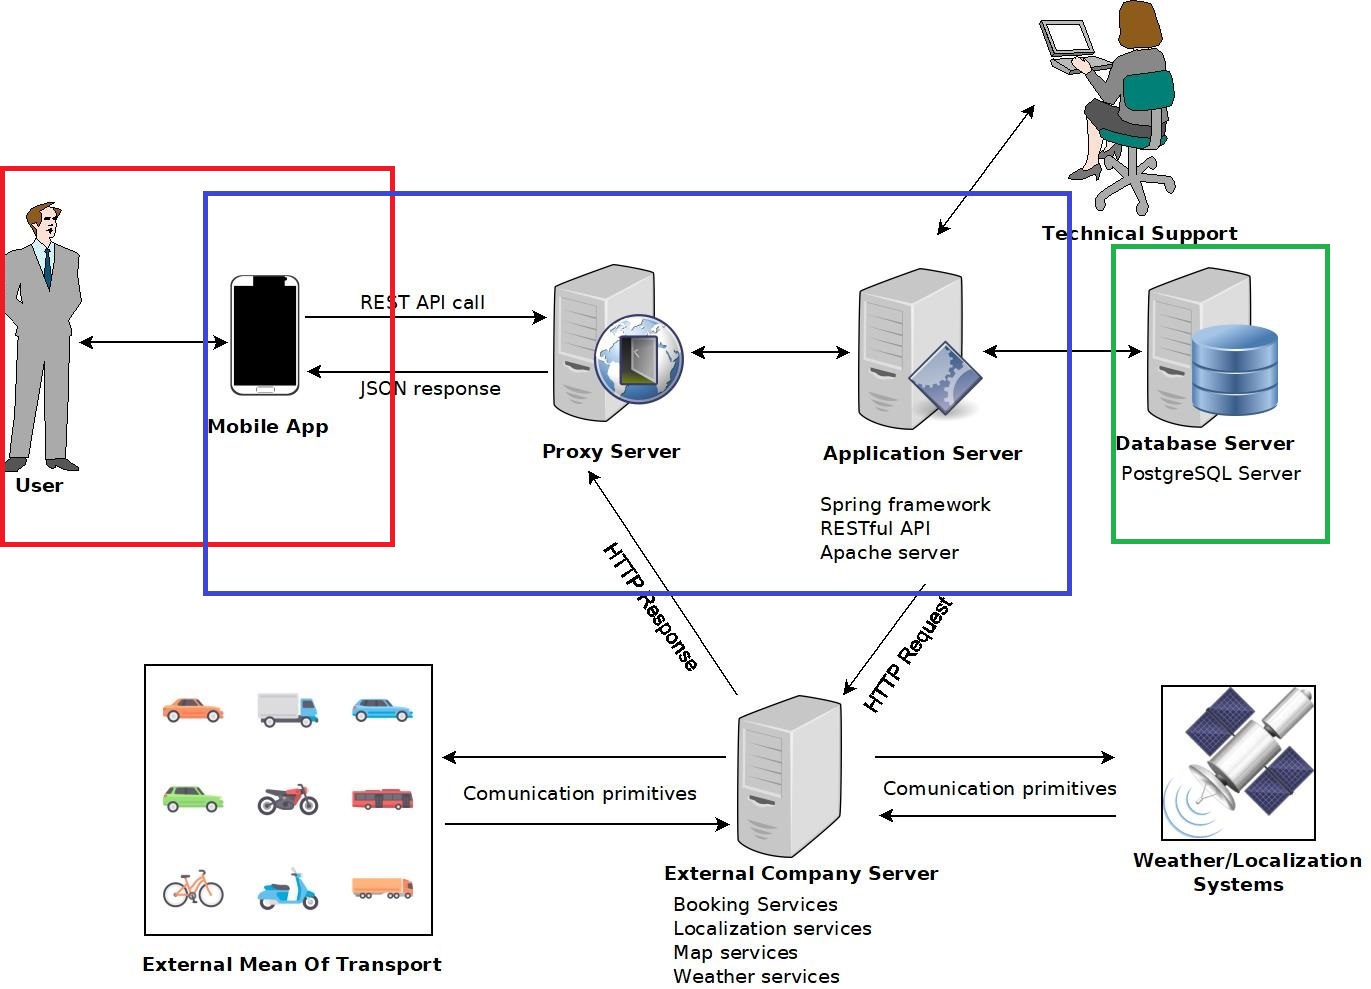
\includegraphics[scale=0.3]{ProposedSystemDiagram_17112017_1}
	\end{centering}
	\caption{Proposed system with tier division. Red: presentation, Blue: logic, Green: data}
\end{figure}

The presentation layer consists of the mobile application, which provides a GUI for the interaction of the user with the service.\\
The logic layer is mainly represented by the application server, where all main decisions and computation take place, although a small part of logic is left to the mobile application (simple elaborations of data such as the location of the user through GPS, or remodeling of the view presented to the user).\\
A proxy server is inserted between the application server and the mobile application for security reasons.\\
Finally, the data layer is represented by the database server, interacting with the application server when needed.

\subsection{Component view}
\subsection{Deployment view}
\subsection{Runtime view}
\subsection{Component Interfaces}
\subsection{Selected architectural styles and patterns}
\subsection{Other design decisions}

\newpage
\section{Algorithm design}

\newpage
\section{User interface design}

\newpage
\section{Requirements traceability}

\newpage
\section{Implementation, integration and test plan}

\newpage
\section{Effort spent}

\newpage
\section{References}
	
\end{document}